\documentclass[a4j]{ltjsarticle}
\usepackage{bookmark}
\usepackage{xurl}
\usepackage{enumerate}
% 数式
\usepackage{luatexja}
\usepackage{amsmath,amsfonts,amssymb,ascmac}
\usepackage{bm}
\usepackage{url}
\usepackage{mathtools}
\usepackage[shortlabels]{enumitem}
\usepackage{mathrsfs}
\usepackage{tikz}
\usetikzlibrary{cd}
\setcounter{tocdepth}{3}
\newcommand{\Rset}{\mathbb{R}}
\newcommand{\Nset}{\mathbb{N}}
\newcommand{\Zset}{\mathbb{Z}}
\newcommand{\Qset}{\mathbb{Q}}
\newcommand{\Cset}{\mathbb{C}}
\newcommand{\transpose}[1]{\prescript{t\!}{}{#1}}
\mathtoolsset{showonlyrefs=true}
\numberwithin{equation}{section}
\usepackage{physics}
% 画像
\usepackage{graphicx}

% 定理環境
\usepackage{amsthm}
\theoremstyle{definition}
\newtheorem{thm}{定理}[section]
\newtheorem{cor}[thm]{系}
\newtheorem{dfn}[thm]{定義}
\newtheorem{prop}[thm]{命題}
\newtheorem{lem}[thm]{補題}
\newtheorem{rmk}[thm]{注意}
\newtheorem{eg}[thm]{例}

\begin{document}
\title{極小曲面入門---セッケン膜の形の数理---}
\author{un cinglé}
\date{}
\maketitle
\section{はじめに}
柄のついた円形の針金を2つ用意し,これらを重ねてセッケン液に浸したのち引き上げると,その間には少しくびれた,特徴的な形状のセッケン膜が張られる.フレームの形を変えてみると別の形が現れて面白いだろう.セッケン膜の美しい形に魅入られた建築家F. Ottoは,ドイツ・パビリオン(1962年)やミュンヘンオリンピック競技場(1972年)といった作品で屋根にセッケン膜を模した造形を用いた(参考文献\cite{HT},\cite{FB}).なお,円形フレームに張られるセッケン膜はカテノイド(懸垂面)と呼ばれる曲面であることが知られている.

\begin{figure}[htbp]
    \begin{center}
        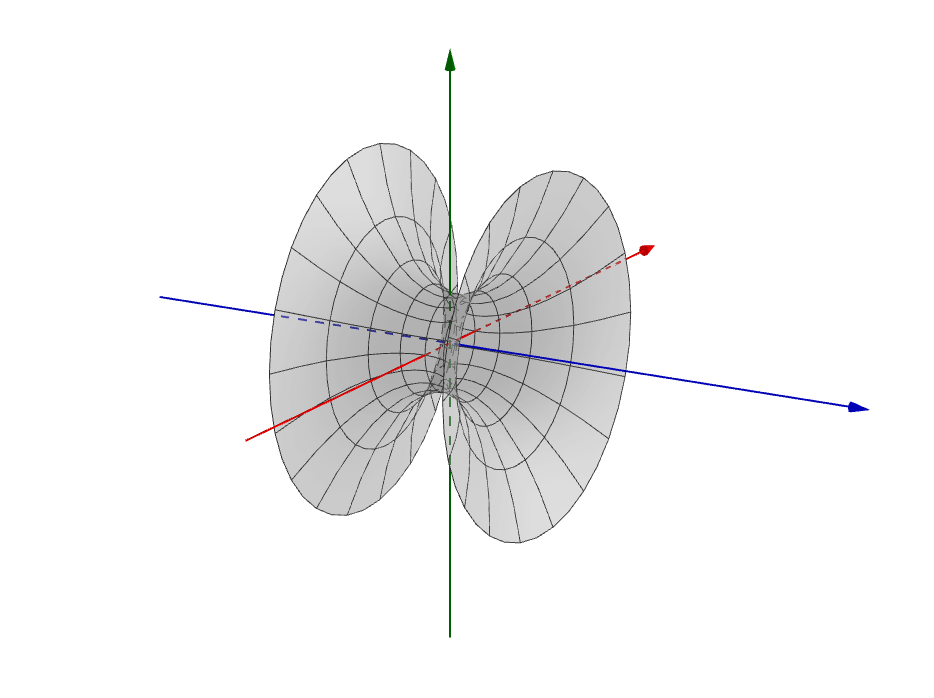
\includegraphics[height=50mm]{catenoid.png}
        \label{pic:catenoid}
        \caption{カテノイド}
    \end{center}
\end{figure}

セッケン膜の形は子どもたちや建築家のみならず,数学者の関心の的でもある.セッケン膜は``極小曲面''と呼ばれるクラスの曲面を形成することが知られている(実はカテノイドも極小曲面の一種である).極小曲面の名前の由来は``面積が極小''ということである(正確な意味はここでは述べない).セッケン膜の表面には表面張力という力が働いており,それは表面積をなるべく小さくするように作用する.その結果,セッケン膜の形状は極小曲面で安定するのである.「与えられた閉曲線に対してそれを境界に持つ極小曲面を決定せよ」という所謂``Plateau問題''は現在においても大変な難問である.

本論では,まず平均曲率を用いて極小曲面を数学的に定義し,それが表面積極小という条件で特徴づけられることを変分法を用いて示す.その後,極小曲面を作り出す``Weierstrass--Enneperの表現公式''を紹介し,例をもって極小曲面たちに親しんでもらうことにする.

\section{曲面論ショートコース}
本節では以下の議論で必要な最低限の曲面論を述べる.目標は,平均曲率を定義することである.
\begin{dfn}\label{dfn:curve}
    $(u,v)$-平面$\Rset^2$の領域$D$から$\Rset^3$への$C^\infty$級写像$p:D\to \Rset^3$であって,$D$の各点で$p$の$u,v$偏微分(これらをそれぞれ$p_u,p_v$と記す)が一次独立であるようなものを,(正則)曲面という.
\end{dfn}
\begin{dfn}\label{dfn:1st}
    $p=p(u,v):D\to \Rset^3$を曲面とする.これに対して行列$I$および(スカラー)量$E,F,G$を
    \begin{equation}
        I\coloneq \begin{bmatrix}
            E & F\\
            F & G 
        \end{bmatrix}\coloneq \begin{bmatrix}
            p_u\cdot p_u & p_u\cdot p_v \\
            p_v\cdot p_u & p_v\cdot p_v
        \end{bmatrix} 
    \end{equation}
    とおく($\;\cdot\;$は内積).$I$を\textbf{第1基本行列}といい,$E,F,G$を\textbf{第1基本量}という.
\end{dfn}
\begin{rmk}
    第1基本行列の行列式を計算してみると,
    \begin{equation}
        \det I=EG-F^2=\abs{p_u}^2\abs{p_v}^2-(p_u\cdot p_v)^2=\abs{p_u\times p_v}^2\label{eq:det_1st}
    \end{equation}
    である($\;\times\;$は外積).いま$p_u,p_v$は一次独立なので$EG-F^2=\abs{p_u\times p_v}^2>0$である.
\end{rmk}
\begin{dfn}
    曲面$p:D\to \Rset^3$に対して 
    \begin{equation}
        \nu\coloneq \frac{p_u\times p_v}{\abs{p_u\times p_v}}
    \end{equation}
    とおくと,$D$の各点$(u,v)$において$\nu(u,v)$は$p_u(u,v),p_v(u,v)$に直交する長さ1のベクトルである.$\nu$を曲面$p$の\textbf{単位法ベクトル場}という.
\end{dfn}
\begin{dfn}
    $p=p(u,v):D\to \Rset^3$を曲面とする.これに対して行列$I\!I$および(スカラー)量$L,M,N$を
    \begin{equation}
        I\!I\coloneq \begin{bmatrix}
            L & M\\
            M & N 
        \end{bmatrix}\coloneq \begin{bmatrix}
            p_{uu}\cdot \nu & p_{uv}\cdot \nu \\
            p_{vu}\cdot \nu & p_{vv}\cdot \nu
        \end{bmatrix} 
    \end{equation}
    とおく.$I\!I$を\textbf{第2基本行列}といい,$L,M,N$を\textbf{第2基本量}という.
\end{dfn}
\begin{dfn}
    以下で定義される行列$A$を\textbf{Weingarten行列}という.
    \begin{equation}
        A\coloneq I^{-1}I\!I=\frac{1}{EG-F^2}\begin{bmatrix}
            G & -F\\
            -F & E
        \end{bmatrix}\begin{bmatrix}
            L & M\\
            M & N
        \end{bmatrix}=\frac{1}{EG-F^2}\begin{bmatrix}
            GL-FM & GM-FN\\
            -FL+EM & -FM+EN
        \end{bmatrix}
    \end{equation}
    また,
    \begin{equation}
        K\coloneq \det A=\frac{LN-M^2}{EG-F^2},\quad H\coloneq \frac{1}{2}\tr A=\frac{EN-2FM+GL}{2(EG-F^2)}
    \end{equation}
    とおき,$K$を\textbf{Gauss曲率},$H$を\textbf{平均曲率}という.
\end{dfn}
\begin{dfn}
    各点で平均曲率が0となる,つまり$H=0$である曲面を\textbf{極小曲面}という.
\end{dfn}
\section{表面積の変分と平均曲率}
第1節で述べたように,セッケン膜はその表面に働く表面張力の効果により,表面積が``極小''となる曲面で安定する.本節では,表面積が極小であるということを``変分法''と呼ばれる手法を用いて定式化し,セッケン膜が極小曲面となることを示す.
\subsection{表面積を求める公式}
まず準備として,曲面の表面積が第1基本量で書けることを示す.以下$p:D\to \Rset^3$を曲面とする.

$(u,v)\in D$とする.$0<\varDelta u,\varDelta v\ll 1$として,$D$内の微小長方形領域$[u,u+\varDelta u]\times [v,v+\varDelta v]$に対応する曲面部分の面積を$\varDelta S$とする.Taylorの定理より
\begin{align}
    p(u+\varDelta u,v)-p(u,v)&\approx p_u(u,v)\varDelta u,\\
    p(u,v+\varDelta v)-p(u,v)&\approx p_v(u,v)\varDelta v
\end{align}
なので,$\varDelta S$は
\begin{equation}
    p(u,v),\quad p(u,v)+p_u(u,v)\varDelta u,\quad p(u,v)+p_v(u,v)\varDelta v,\quad p(u,v)+p_u(u,v)\varDelta u+p_v(u,v)\varDelta v
\end{equation}
を4頂点にもつ平行四辺形の面積で近似できる.したがって 
\begin{equation}
    \varDelta S\approx \abs{(p_u(u,v)\varDelta u)\times (p_v(u,v)\varDelta v)}=\abs{p_u(u,v)\times p_v(u,v)}\varDelta u\varDelta v=\sqrt{EG-F^2}\varDelta u\varDelta v
\end{equation}
を得る(\eqref{eq:det_1st}式を用いた).表面積$S$は$D$上でこの微小面積を足し合わせて得られるので
\begin{equation}
    S=\iint_{D}\sqrt{EG-F^2}dudv=\iint_{D}\sqrt{\det I}dudv
\end{equation}
と求まる.
\subsection{表面積の変分}
``表面積が極小''ということの意味を明確にしよう.

曲面$p=p(u,v)$が与えられたとき,新たな変数$s$による曲面の族$\widetilde{p}(s;u,v)$を考える.ただし,
\begin{itemize}
    \item $\widetilde{p}(0;u,v)=p(u,v)$,
    \item 変分は境界を保つ.つまり$\widetilde{p}(s;u,v)=p(u,v)\quad ((u,v)\in \partial D)$.
\end{itemize}
を仮定する.これを曲面$p$の\textbf{変分}という.$s$を固定したとき曲面$\widetilde{p}(s;u,v)$の表面積を$\widetilde{S}(s)$とおく.もし曲面$p$において表面積が極小となるなら,実数$s$の関数$\widetilde{S}(s)$は$s=0$において極小となる,よって 
\begin{equation}
    \left.\frac{d}{ds}\right|_{s=0}\widetilde{S}(s)=0\label{eq:variation}
\end{equation}
となるはずである.一般に,任意の変分$\widetilde{p}(s;-)$に対して\eqref{eq:variation}式が成り立つこととして表面積が極値を取るということを``定義''する.
\begin{equation}
    V(u,v)\coloneq \left.\frac{d}{ds}\right|_{s=0}\widetilde{p}(s;u,v)
\end{equation}
とおき,これを\textbf{変分ベクトル場}という.

まず,$\widetilde{E}_s=(\widetilde{p}_u\cdot \widetilde{p}_u)_s=2\widetilde{p}_{us}\cdot \widetilde{p}_u$より$\widetilde{E}_s(0)=2V_u\cdot p_u$である.同様に
\begin{equation}
    \widetilde{E}_s(0)=2V_u\cdot p_u,\quad \widetilde{F}_s(0)=V_u\cdot p_v+V_v\cdot p_u,\quad \widetilde{G}_s(0)=2V_v\cdot p_v 
\end{equation}
である.
\begin{equation}
    \frac{d}{ds}(\det \widetilde{I})=\frac{d}{ds}(\widetilde{E}\widetilde{G}-\widetilde{F}^2)=\widetilde{E}\widetilde{G}_s+\widetilde{E}_s\widetilde{G}-2\widetilde{F}\widetilde{F}_s
\end{equation}
より,とくに$s=0$として 
\begin{equation}
    \left.\frac{d}{ds}\right|_{s=0}(\det \widetilde{I})=2(E(V_v\cdot p_v)+G(V_u\cdot p_u)-F(V_u\cdot p_v+V_v\cdot p_u))
\end{equation}
を得る.したがって,
\begin{equation}
    \left.\frac{d}{ds}\right|_{s=0}\sqrt{\det \widetilde{I}}=\frac{E(V_v\cdot p_v)+G(V_u\cdot p_u)-F(V_u\cdot p_v+V_v\cdot p_u)}{\sqrt{\det I}}
\end{equation}
ここで積の微分公式より
\begin{equation}
    \frac{E(V_v\cdot p_v)}{\sqrt{\det I}}=\qty(\frac{E}{\sqrt{\det I}}(V\cdot p_v))_v-V\cdot \qty(\frac{E}{\sqrt{\det I}}p_v)_v
\end{equation}
である.他の項についても同様の計算をして整理すると
\begin{align}
    \begin{split}
        &\quad \left.\frac{d}{ds}\right|_{s=0}\sqrt{\det \widetilde{I}}\\
    &=\qty(\frac{E}{\sqrt{\det I}}(V\cdot p_v))_v+\qty(\frac{G}{\sqrt{\det I}}(V\cdot p_u))_u-\qty(\frac{F}{\sqrt{\det I}}(V\cdot p_v))_u-\qty(\frac{F}{\sqrt{\det I}}(V\cdot p_u))_v\\
    &\quad -V\cdot \qty(\qty(\frac{E}{\sqrt{\det I}}p_v)_v+\qty(\frac{G}{\sqrt{\det I}}p_u)_u-\qty(\frac{F}{\sqrt{\det I}}p_v)_u-\qty(\frac{F}{\sqrt{\det I}}p_u)_v)
    \end{split}\label{eq:der_area_element}
\end{align}
となる.まず下段の括弧の中身を計算しよう.結果は次のようになる.
\begin{prop}\label{prop:prep1}
    \begin{equation}
        \qty(\frac{E}{\sqrt{\det I}}p_v)_v+\qty(\frac{G}{\sqrt{\det I}}p_u)_u-\qty(\frac{F}{\sqrt{\det I}}p_v)_u-\qty(\frac{F}{\sqrt{\det I}}p_u)_v=2H\sqrt{\det I}\;\nu.
    \end{equation}
\end{prop} 
\begin{proof}
    左辺を$N$とおく.まず$N$が$p_u,p_v$と直交することを示す.再び積の微分より
    \begin{align}
        p_u\cdot N&=\qty(p_u\cdot \frac{E}{\sqrt{\det I}}p_v)_v-p_{uv}\cdot \frac{E}{\sqrt{\det I}}p_v+\qty(p_u\cdot \frac{G}{\sqrt{\det I}}p_u)_u-p_{uu}\cdot \frac{G}{\sqrt{\det I}}p_u\\
        &\quad -\qty(p_u\cdot \frac{F}{\sqrt{\det I}}p_u)_v+p_{uv}\cdot \frac{F}{\sqrt{\det I}}p_u-\qty(p_u\cdot \frac{F}{\sqrt{\det I}}p_v)_u+p_{uu}\cdot \frac{F}{\sqrt{\det I}}p_v
    \end{align}
    となるが,第1基本量の定義より第1項と第5項は打ち消し合って消える.また第3項と第7項を合わせると$(\sqrt{\det I})_u$となる.第偶数項を全部足すと
    \begin{align}
        &\quad -\frac{E(p_{uv}\cdot p_v)+G(p_{uu}\cdot p_u)-F(p_{uv}\cdot p_u+p_{uu}\cdot p_v)}{\sqrt{\det I}}\\
        &=-\frac{E(p_v\cdot p_v)_u-F((p_u\cdot p_v)_u+(p_v\cdot p_u)_u)+G(p_u\cdot p_u)_u}{2\sqrt{\det I}}\\
        &=-\frac{EG_u-2FF_u+GE_u}{2\sqrt{\det I}}\\
        &=-\frac{(\det I)_u}{2\sqrt{\det I}}=-(\sqrt{\det I})_u
    \end{align}
    となる.以上をあわせると$p_u\cdot N=0$を得る.同様に$p_v\cdot N=0$である.よって$N$は$p_u,p_v$と直交するので$\nu$と平行である.
    \begin{equation}
        N=(N\cdot \nu)\nu=\qty(\frac{Ep_{vv}-2Fp_{uv}+Gp_{uu}}{\sqrt{\det I}}\cdot \nu)\nu=\frac{EN-2FM+GL}{\sqrt{\det I}}\nu =2H\sqrt{\det I}\;\nu
    \end{equation}
    より結論を得る.
\end{proof}
次に\eqref{eq:der_area_element}式の第1から第4項までの和を計算しよう.
\begin{prop}\label{prop:prep2}
    $V=V_1p_u+V_2p_v+V_3\nu$とおく.このとき 
    \begin{align}
        &\quad \qty(\frac{E}{\sqrt{\det I}}(V\cdot p_v))_v+\qty(\frac{G}{\sqrt{\det I}}(V\cdot p_u))_u-\qty(\frac{F}{\sqrt{\det I}}(V\cdot p_v))_u-\qty(\frac{F}{\sqrt{\det I}}(V\cdot p_u))_v\\
        &=\qty(\sqrt{\det I}\; V_1)_u+\qty(\sqrt{\det I}\;V_2)_v.
    \end{align}
\end{prop}
\begin{proof}
    $V=V_1p_u+V_2p_v+V_3\nu$と第1基本量の定義より 
    \begin{align}
        \qty(\frac{E}{\sqrt{\det I}}(V\cdot p_v))_v&=\qty(\frac{E(V_1F+V_2G)}{\sqrt{\det I}})_v,& \qty(\frac{G}{\sqrt{\det I}}(V\cdot p_u))_u=\qty(\frac{G(V_1E+V_2F)}{\sqrt{\det I}})_u,\\
        \qty(\frac{F}{\sqrt{\det I}}(V\cdot p_v))_u&=\qty(\frac{F(V_1F+V_2G)}{\sqrt{\det I}})_u,& \qty(\frac{F}{\sqrt{\det I}}(V\cdot p_u))_v=\qty(\frac{F(V_1E+V_2F)}{\sqrt{\det I}})_v
    \end{align}
    である.これを用いて示すべき式の左辺を$u,v$偏微分の項ごとにまとめると
    \begin{equation}
        \qty(\frac{EG-F^2}{\sqrt{\det I}}V_1)_u+\qty(\frac{EG-F^2}{\sqrt{\det I}}V_2)_v=\qty(\sqrt{\det I}\; V_1)_u+\qty(\sqrt{\det I}\;V_2)_v
    \end{equation}
    となって結論を得る.
\end{proof}
命題\ref{prop:prep1},\ref{prop:prep2}の結果と\eqref{eq:der_area_element}式より
\begin{equation}
    \left.\frac{d}{ds}\right|_{s=0}\sqrt{\det \widetilde{I}}=\qty(\sqrt{\det I}\; V_1)_u+\qty(\sqrt{\det I}\;V_2)_v-2(V\cdot \nu)H\sqrt{\det I}\label{eq:beautiful}
\end{equation}
を得る.
\begin{thm}[第1変分公式]\label{thm:var_formula}
    \begin{equation}
        \left.\frac{d}{ds}\right|_{s=0}\widetilde{S}(s)=-2\iint_{D}(V\cdot \nu) H\sqrt{\det I}\;dudv.
    \end{equation}
\end{thm}
\begin{proof}
    積分と微分の順序交換をして\eqref{eq:beautiful}式を用いると
    \begin{align}
        \left.\frac{d}{ds}\right|_{s=0}\sqrt{\det \widetilde{I}}&=\iint_{D}\left.\frac{d}{ds}\right|_{s=0}\sqrt{\det \widetilde{I}}\;dudv \\
        &=\iint_{D}\qty(\qty(\sqrt{\det I}\; V_1)_u+\qty(\sqrt{\det I}\;V_2)_v)dudv-2\iint_{D}(V\cdot \nu)H\sqrt{\det I}\;dudv
    \end{align}
    である.上の第1項が0であることを示せば証明が完了する.Greenの公式より,
    \begin{equation}
        \iint_{D}\qty(\qty(\sqrt{\det I}\; V_1)_u+\qty(\sqrt{\det I}\;V_2)_v)dudv=\int_{\partial D}\sqrt{\det I}\;(-V_2du+V_1dv)
    \end{equation}
    だが,変分が境界を保つという条件より$\partial D$上$V=0$だから右辺は0となる.以上より結論を得る.
\end{proof}
\subsection{極小曲面と表面積}
\begin{lem}
    $D$を領域,$(u_0,v_0)$を$D$の内点とする.このとき,$D$上の$C^\infty$級関数$\varphi:D\to\Rset$で次を満たすものが存在する:$\varphi=\varphi_u=\varphi_v=0\ \text{on $\partial D$},\quad \varphi(u_0,v_0)>0$.
\end{lem}
\begin{proof}
    $R>0$を十分小さく取って$(u_0,v_0)$中心,半径$2R$の円板が$D$に含まれるようにする.この円板を$B$と名付ける. 
    \begin{equation}
        f(t)\coloneq \begin{cases}
            e^{-1/t^2} & (t>0)\\
            0 & (t\leq0)
        \end{cases},\quad g(t)\coloneq \frac{f(t)}{f(t)+f(1-t)},
    \end{equation}
    \begin{equation}
        \varphi(u,v)\coloneq \begin{cases}
            g\qty(1-\frac{(u-u_0)^2+(v-v_0)^2}{R^2}) & ((u,v)\in B)\\
            0 & ((u,v)\notin B)
        \end{cases}
    \end{equation}
    とおくと$\varphi$が条件を満たす.
\end{proof}
\begin{thm}
    曲面について,表面積が極値を取る(任意の変分に対して$\left.\frac{d}{ds}\right|_{s=0}\widetilde{S}=0$)であることと,極小曲面であることは同値である.
\end{thm}
\begin{proof}
    定理\ref{thm:var_formula}より極小曲面なら表面積は極値を取る.逆に$p$を表面積が極値を取るとする.$D$の内点$(u_0,v_0)$を1つ固定する.1つ前の補題の$\varphi$を取り,ベクトル場$V$を$V\coloneq \varphi H \nu$で定める.変分$\widetilde{p}(s;u,v)\coloneq p+sV$を考えるとその変分ベクトル場は$V$である.再び定理\ref{thm:var_formula}より 
    \begin{equation}
        \left.\frac{d}{ds}\right|_{s=0}\widetilde{S}(s)=-2\iint_{D}(V\cdot \nu) H\sqrt{\det I}\;dudv=-2\iint_{D}H^2\sqrt{\det I}\; dudv 
    \end{equation}
    となるが,これが0なので$(u_0,v_0)$で$H=0$とならざるを得ない.$(u_0,v_0)$は任意なので結論を得る.
\end{proof}
この定理こそが``極小曲面''という名前の謂である.セッケン膜は表面張力の効果で表面積が極小になるような形状を取り,したがって平均曲率0の極小曲面を形成する.
\section{極小曲面を作って遊ぼう}
\subsection{回転面である極小曲面}
円形のフレームに張られるセッケン膜は,回転対称な形をしているはずであろう.そこで,まずは回転面であるような極小曲面を決定する.

$xz$-平面内の曲線$(x(u),z(u)),\ x(u)>0$を$y$軸回りに回転させてできる回転面を$p$とする.ただし,曲線は速さが1である,すなわち
\begin{equation}
    (x'(u))^2+(z'(u))^2=1\label{eq:len_para}
\end{equation}
であると仮定する(このとき$u$は\textbf{弧長パラメータ}であるという).回転面$p$のパラメータ表示は
\begin{equation}
    p(u,v)=\begin{bmatrix}
        x(u)\cos v\\
        x(u)\sin v\\
        z(u) 
    \end{bmatrix}
\end{equation}
で与えられる.計算の詳細は省くが,平均曲率$H$は$H=\frac{1}{2}\qty(x''z'-x'z''-\frac{z'}{x})$である.よって,$p$が極小曲面であるための条件は
\begin{equation}
    x''z'-x'z''-\frac{z'}{x}=0.\label{eq:min_surf_rot}
\end{equation}
また\eqref{eq:len_para}式を微分して
\begin{equation}
    x'x''+z'z''=0\label{eq:len_para_der}
\end{equation}
を得る.$(x')^2+(z')^2=1$に注意して$\text{\eqref{eq:min_surf_rot}}\times z'+\text{\eqref{eq:len_para_der}}\times x'$を計算すると$(xx')'=xx''+(x')^2=1$を得る.よって$(x^2/2)'=xx'=u+c_1$となり$x^2=u^2+2c_1u+c_2$となる.平行移動により$c_1=0$としてよく,定数を取り直すことで$x=\sqrt{u^2+a^2}$と書ける.

$\text{\eqref{eq:len_para_der}}\times z'-\text{\eqref{eq:min_surf_rot}}\times x'$より$z''+\frac{u}{u^2+a^2}z'=0$となる.これを解いて\eqref{eq:len_para}式に注意すると$z'=\frac{a}{\sqrt{u^2+a^2}},\ z=a\log(u+\sqrt{u^2+a^2})$となる(平行移動により任意定数は0としてよい).これで$x,z$が$u$の式で書けたわけだが,これらの式から$u$を消去して
\begin{equation}
    \frac{x}{a}=\frac{e^{(z+a\log a)/a}+e^{-(z+a\log a)/a}}{2}
\end{equation}
という関係を得る.よって曲線$(x,z)$は相似変換と平行移動で$x=\frac{e^z+e^{-z}}{2}$と一致するので\textbf{カテナリー}(懸垂線)である.カテナリーの回転面を\textbf{カテノイド}(懸垂面)と呼ぶ.

以上より,回転対称な極小曲面はカテノイドしかないことが示された.これがセッケン膜がカテノイドとなる理由である.
\subsection{Weierstrass--Enneperの表現公式}
本節では一部で簡単な複素関数論の知識を仮定する.

前節で極小曲面のうち回転面であるものは本質的には1種類しかないことがわかった.読者は極小曲面はあまり多くあるわけではないと思われるかもしれないが,実はそうではない.以下に示すように回転面に限らなければ極小曲面はたくさん存在し,それらを具体的に表示する式も知られている.

まず,我々の議論にとって都合の良い座標系を取ることから始める.次の定理の証明は(難しいので)しない.参考文献\cite[定理15.4]{山田}を参照せよ.
\begin{thm}
    $p:D\to \Rset^3$を曲面とする.このとき,$D$の各点に対して,その十分小さい近傍上の座標系$(u,v)$であって,第1基本量が$E=G,F=0$となるようなものが取れる.そのような座標系を\textbf{等温座標系}という.
\end{thm}
そこで,以下曲面は等温座標系で表示されているものとする.
\begin{prop}
    等温座標表示された曲面$p$について,$p$が極小曲面であることと
    \begin{equation}
        p_{uu}+p_{vv}=0\label{eq:harmonic}
    \end{equation}
    が成り立つことは同値である.\eqref{eq:harmonic}式が成り立つとき$p$は\textbf{調和}であるという.
\end{prop}
\begin{proof}
    $E=G,F=0$より第1基本行列がスカラー行列であることに注意すると
    \begin{equation}
        H=\frac{1}{2E}(L+N)=\frac{1}{2E}(p_{uu}+p_{vv})\cdot \nu .
    \end{equation}
    ここで$p_{uu}+p_{vv}$が$\nu$と平行であることが示されれば,$H=0$と$p_{uu}+p_{vv}=0$が同値となり結論が得られる.
    \begin{align}
        p_{uu}\cdot p_{u}&=\frac{1}{2}(p_u\cdot p_u)_u=\frac{1}{2}E_u,\\
        p_{vv}\cdot p_{u}&=(p_{v}\cdot p_u)_v-\frac{1}{2}(p_v\cdot p_v)_u=F_v-\frac{1}{2}G_u=-\frac{1}{2}G_{u}
    \end{align}
    より$(p_{uu}+p_{vv})\cdot p_u=\frac{1}{2}(E_u-G_u)=0$.同様に$(p_{uu}+p_{vv})\cdot p_v=0$である.
\end{proof}
複素関数論によると,$p$が調和であることと$\xi\coloneq p_u-ip_v$が$z=u+iv$に関する正則関数であることは同値である.

次に等温座標である($E=G, F=0$)という条件について考える.$p_u=\frac{\xi+\overline{\xi}}{2},\ p_v=\frac{i(\xi-\overline{\xi})}{2}$より
\begin{equation}
    E=p_u\cdot p_u=\frac{\xi\cdot \xi+2\xi\cdot \overline{\xi}+\overline{\xi}\cdot \overline{\xi}}{4},\quad F=p_u\cdot p_v=\frac{i(\xi\cdot \xi-\overline{\xi}\cdot \overline{\xi})}{4},\quad G=p_v\cdot p_v=-\frac{\xi\cdot \xi-2\xi\cdot \overline{\xi}+\overline{\xi}\cdot \overline{\xi}}{4}
\end{equation}
であるから,等温座標であるための条件は$\xi\cdot \xi=0$である.

したがって,\textbf{極小曲面を求めよ,という問題は「$\xi\cdot \xi=0$を満たす正則関数$\xi=(\xi_1,\xi_2,\xi_3)$を求めよ」という問題に帰着する}.

以上で次の定理を述べる準備ができた.
\begin{thm}[Weierstrass--Enneperの表現公式]
    任意の極小曲面$p=(x,y,z):D\to\Rset^3$は,局所的には正則関数$f$と有理型関数$g$を用いて
    \begin{align}
        x=\Re\int_{z_0}^z 2fgdz,\quad y=\Re\int_{z_0}^z f(1-g^2)dz,\quad z=\Re\int_{z_0}^z if(1+g^2) dz
    \end{align}
    と表される.なお,$f$の零点と$g$の極は一致し,$f$の零点としての位数は$g$の極としての位数の2倍に等しい.逆に上で与えられる曲面は極小曲面である.
\end{thm}
\begin{proof}
    $\xi\coloneq (\xi_1,\xi_2,\xi_3)=p_u-ip_v$とおくと$\xi$は正則で
    \begin{equation}
        \xi\cdot\xi=\xi_1^2+\xi_2^2+\xi_3^2=0\label{eq:isotropic}    
    \end{equation}
    であった.$\xi_1,\xi_2,\xi_3$が全て恒等的に0ならば$p$は曲面とはならないので,例えば$\xi_1\not\equiv0$と仮定する.\eqref{eq:isotropic}式より$\xi_2-i\xi_3\not\equiv0$であり,一致の定理より$\xi_2-i\xi_3$の零点は孤立点である.そこで
    \begin{equation}
        f=\frac{\xi_2-i\xi_3}{2},\quad g=\frac{\xi_1}{\xi_2-i\xi_3}
    \end{equation}
    とおくと$f,g$はそれぞれ正則関数,有理型関数であり,$f$の零点と$g$の極は一致する.また
    \begin{equation}
        \xi_2-i\xi_3=2f,\quad \xi_2+i\xi_3=-\frac{\xi_1^2}{\xi_2-i\xi_3}=-2fg^2
    \end{equation}
    などより$\xi_1=2fg,\ \xi_2=f(1-g^2),\ \xi_3=if(1+g^2)$となる.よって$0<\abs{\xi}^2=2\abs{f}^2\qty(1+\abs{g}^4)$となることから$f$の零点としての位数は$g$の極としての位数の2倍でなければならない.さらに$p_u=\Re (\xi_1,\xi_2,\xi_3)$なので$p$は正則関数$\int_{z_0}^z(\xi_1,\xi_2,\xi_3)dz$の実部になっているはずであり($z_0$は$D$の勝手な点),$p=\Re \int_{z_0}^z (\xi_1,\xi_2,\xi_3)dz$となる.
\end{proof}
\subsection{極小曲面をたくさん作ろう}
Weierstrass--Enneperの表現公式を用いて極小曲面の例を見てみよう.
\begin{eg}[Enneper曲面]
    $f=1,g=z$とすると極小曲面
    \begin{equation}
        p(u,v)=\begin{bmatrix}
            u^2-v^2\\
            u+uv^2-u^3/3\\
            -v-u^2v+v^3/3
        \end{bmatrix}
    \end{equation}
    が得られる.これをEnneper曲面という(図\ref{pic:enneper}).
\end{eg}
\begin{eg}[カテノイド]
    $f=-ie^{-z}/2,g=-ie^{z}$とすると極小曲面
    \begin{equation}
        p(u,v)=\begin{bmatrix}
            -u\\
            \sinh u \sin v\\
            \cosh u \cos v
        \end{bmatrix}
    \end{equation}
    が得られる.これはカテノイドと同じものである(図\ref{pic:catenoid}).
\end{eg}
\begin{eg}[ヘリコイド]
    $f=e^{-z}/2,g=-ie^{z}$とすると極小曲面 
    \begin{equation}
        p(u,v)=\begin{bmatrix}
            v\\
            \sinh u\cos v\\
            \sinh u\sin v 
        \end{bmatrix}
    \end{equation}
    が得られる.これをヘリコイド(常螺旋面)という(図\ref{pic:helycoid}).
\end{eg}
\begin{eg}[Scherk曲面]
    $f=4/(1-z^4),\ g=z$とおくと極小曲面
    \begin{equation}
        p(u,v)=\begin{bmatrix}
            \log\frac{1+2u^2-2v^2+u^4+2u^2v^2+v^4}{1-2u^2+2v^2+u^4+2u^2v^2+v^4}\\
            2\arctan\frac{2u}{1-u^2-v^2}\\
            2\arctan\frac{-2v}{1-u^2-v^2}
        \end{bmatrix}
    \end{equation}
    が得られる.これはScherk曲面と呼ばれ,$e^x=\frac{\cos y}{\cos z}$という陰関数表示を持つ(図\ref{pic:scherk}).
\end{eg}
\begin{figure}[htbp]
    \begin{minipage}{0.45\linewidth}
      \centering
      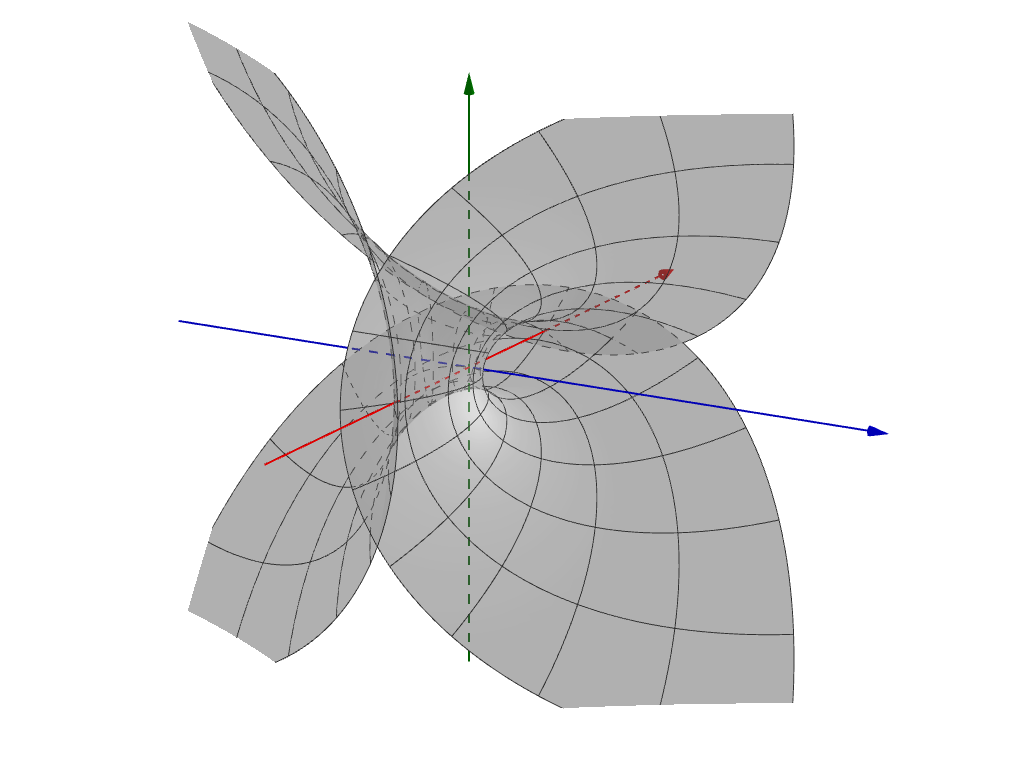
\includegraphics[height=50mm]{enneper.png}
      \caption{Enneper曲面}
      \label{pic:enneper}
    \end{minipage}
    \begin{minipage}{0.45\linewidth}
        \centering
        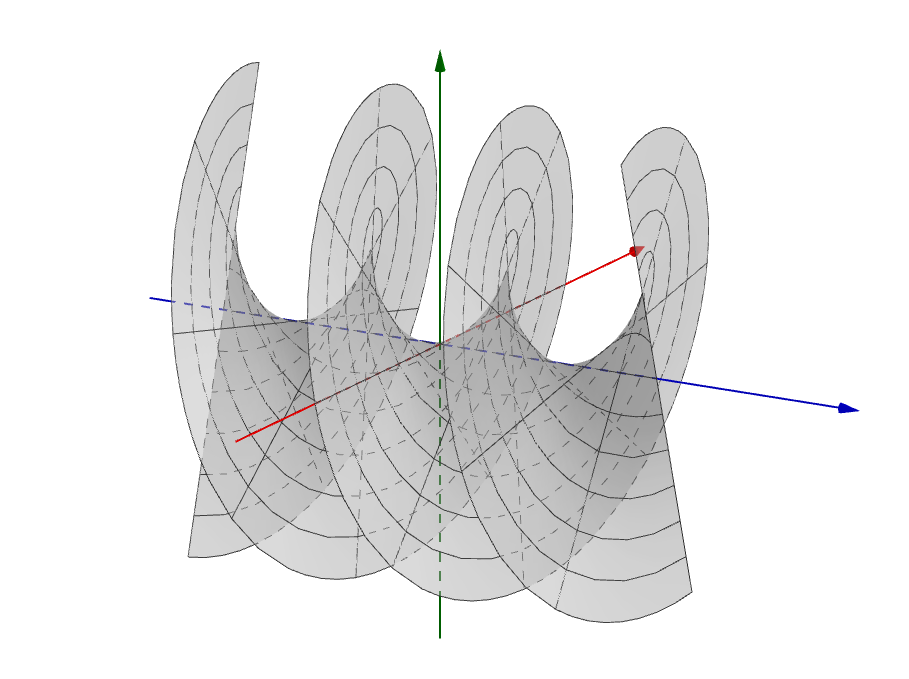
\includegraphics[height=50mm]{helycoid.png}
        \caption{ヘリコイド}
        \label{pic:helycoid}
      \end{minipage}
      \begin{minipage}{0.45\linewidth}
        \centering
        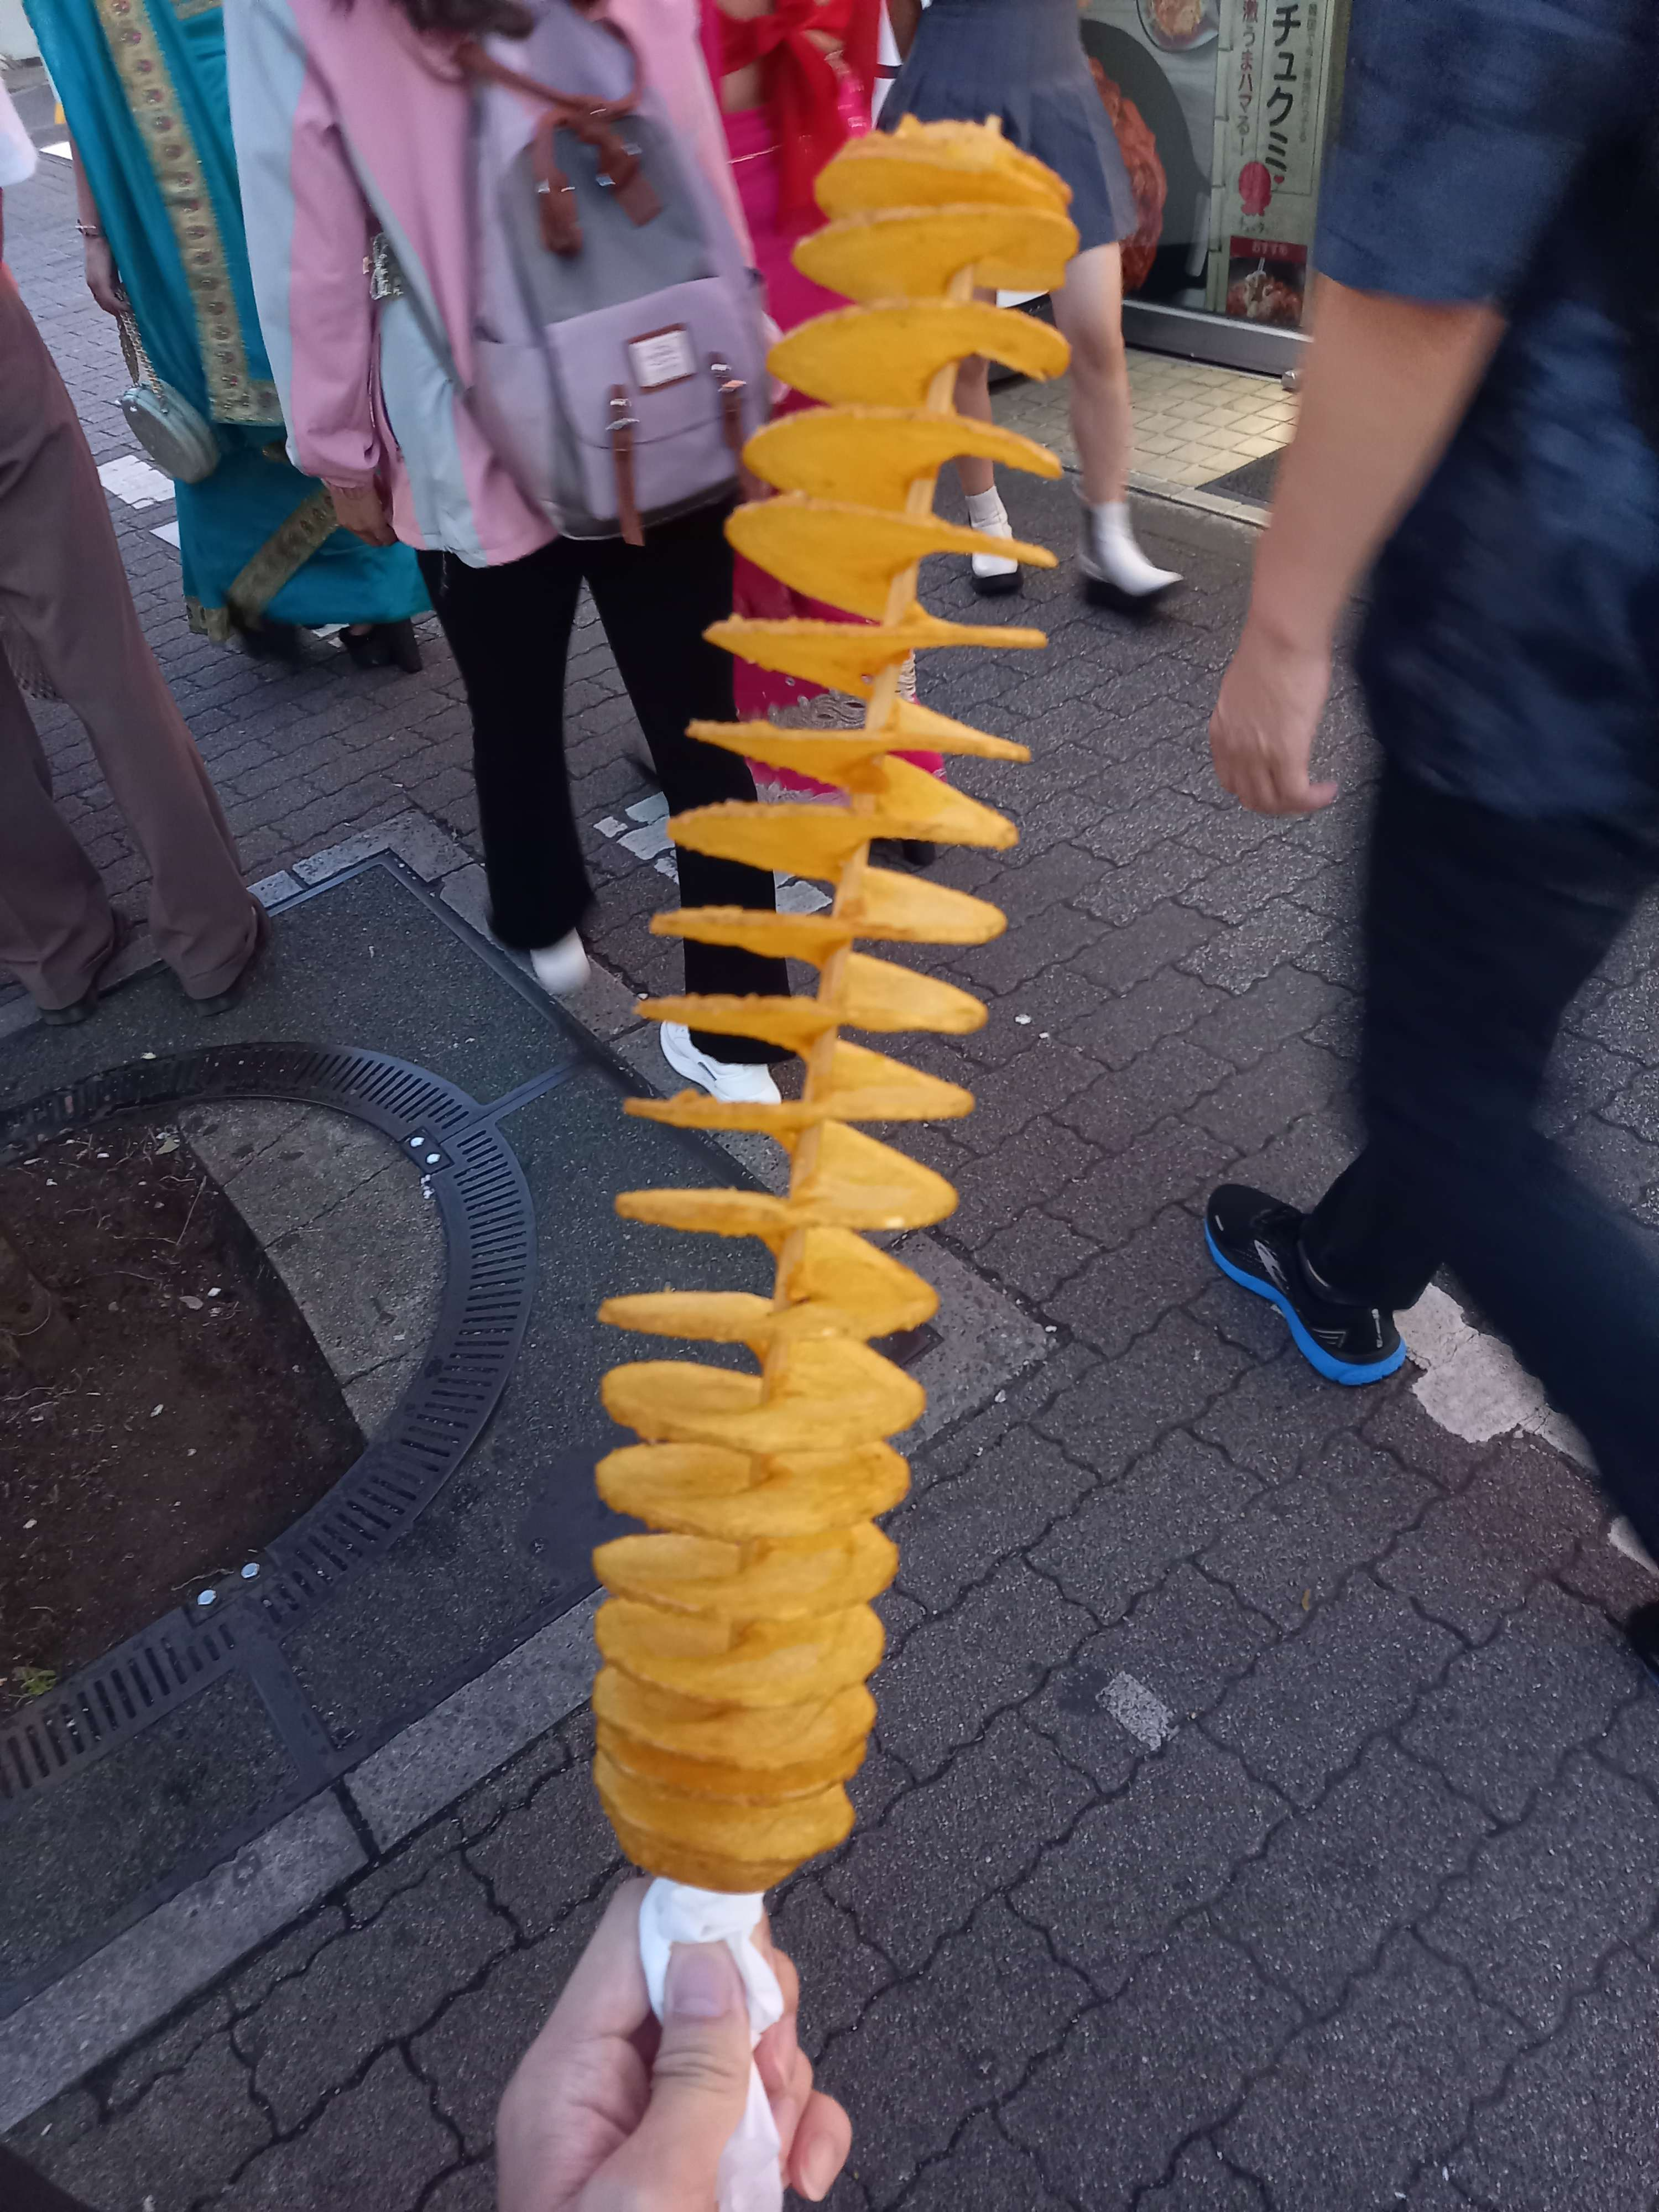
\includegraphics[height=50mm]{twistpotato.jpg}
        \caption{身の回りのヘリコイド(筆者撮影)}
        \label{pic:twistpotato}
      \end{minipage}
      \begin{minipage}{0.45\linewidth}
        \centering
        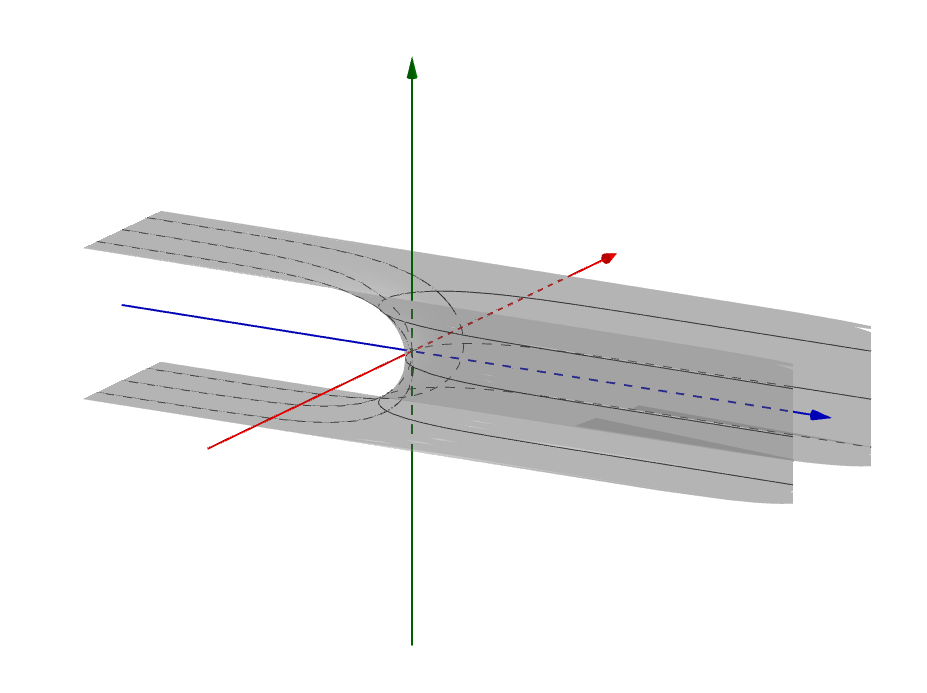
\includegraphics[height=50mm]{scherk.png}
        \caption{Scherk曲面(の一部)}
        \label{pic:scherk}
      \end{minipage}    
\end{figure}
\section{終わりに}
ここまでセッケン膜の形を題材として極小曲面を紹介し,その性質を調べてきた.ここで極小曲面やその周辺の話題で紹介しきれなかったものについて簡単に述べておきたい.

定義\ref{dfn:curve}を見ればわかるように,本稿で扱った極小曲面は全て``正則な''曲面であり,特異点は存在しないもののみを考えた.しかし,実際に作ってみるとわかるが,セッケン膜には特異点が非常に自然に現れる.例えば複数のセッケン膜同士が接触するときにはその接触面に特異点集合が現れる(写真が参考文献\cite{HT},\cite{FB}などにある).これも表面積が極小となるという仮定から導かれる事実なのだが,特異点をもつ曲面について本稿の議論は通用しない.この事情が前述のPlateau問題を非常に難しい問題にしている.

また,本稿では境界を持つセッケン膜について考えたが,読者にとって更に親しみのある現象としてシャボン玉の形があると思う.シャボン玉の表面には同様に表面張力が働くが,セッケン膜とは異なり境界がなく,内部の空気の量が一定であることから体積が一定となる.したがって対応する変分問題は「体積一定の曲面で表面積が最小となるものを求めよ」となる.そしてその解は``平均曲率が0でない一定となる曲面''であることがわかる(参考文献\cite{小磯}).実は「平均曲率一定の閉曲面で,球面と同相なものは球面に限る(Hopfの定理)」,「平均曲率一定の閉曲面で,自己交差のないものは球面に限る(Alexandrov)」ことが知られている(参考文献\cite{井ノ口}).これらはある意味でシャボン玉が丸いことの証明になっている.余談だが,これらの事実が示されたあと「平均曲率一定な閉曲面は球面に限るか?」という所謂``Hopfの問題''が提起されたが,Wenteによって平均曲率一定輪環面が構成されたことにより否定的に解決された(1984年).極小曲面がWeierstrass--Enneperの表現公式で簡潔に表示できたこととは対照的に,平均曲率が0でない一定な曲面の構成は難しい問題である.

以上のようにセッケン膜の問題は本稿で議論したことよりも更に深い内容を含んでいる.興味を持たれた読者は参考文献\cite{山田},\cite{小磯},\cite{井ノ口}に挙げた専門書を開いてみるとよい.また参考文献\cite{HT},\cite{FB}は一般書である.どちらも挿絵が豊富で数式は出てこないので誰にとっても楽しく読むことができる本だと思う.

\begin{thebibliography}{99}
    \bibitem{山田}
    梅原雅顕,山田光太郎著『曲線と曲面---微分幾何的アプローチ---』.裳華房,2015年.

    \bibitem{小磯}
    小磯憲史著『変分問題』.共立出版,1999年.

    \bibitem{井ノ口}
    井ノ口順一著『曲面と可積分系』.朝倉書店,2015年.

    \bibitem{HT}
    ステファン・ヒルデブラント,アンソニー・トロンバ著,小川泰,神志那良雄,平田隆幸訳『形の法則---自然界の形とパターン---』.東京化学同人,1994年.
    \bibitem{FB}
    フィリップ・ボール著,林大訳『かたち 自然が創り出す美しいパターン1』.早川書房,2016年.
\end{thebibliography}

\end{document}